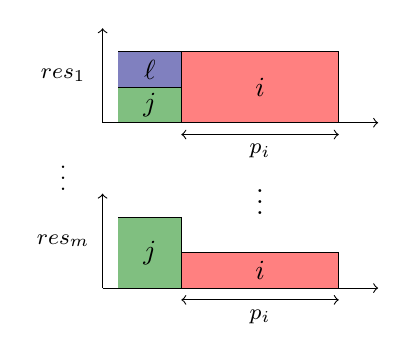
\begin{tikzpicture}
  [yscale=0.3]
  \node[label={[shift={(-0.4,-0.5)}]}] (O) at (0,0) {};
  \draw[fill=red!50] (1,0) rectangle (3,3)   node[midway] {$i$};
  
  \onslide<2-3>{
    \draw[<->] (1,-0.5) -- (3,-0.5) node[midway,below] {\footnotesize $p_i$};
  }
  \onslide<3>{
    \draw[<->] (0.8,0) -- (0.8,3) node[midway,left] {\footnotesize $b_{i1}$};
  }
  
  \draw[->] (O.center) -- (0,4);
  \draw[->] (O.center) -- (3.5,0);


  \onslide<3->{
  \node at (2,-3) {$\vdots$};

  \draw[fill=red!50] (1,-7)rectangle (3,-5.5) node[midway] {$i$};
  
  \onslide<3>{
    \draw[<->] (1,-7.5) -- (3,-7.5) node[midway,below] {\footnotesize $p_i$};
  }
  \onslide<3>{
    \draw[<->] (0.8,-7) -- (0.8,-5.5) node[midway,left]
    {\footnotesize $b_{im}$};
  }
  
  \node at (-0.5,2) {\footnotesize $res_1$};
  \node at (-0.5,-5) {\footnotesize $res_m$};
  \node at (-0.5,-2) {\footnotesize $\vdots$};

  \draw[->] (0,-7) -- (0,-3);
  \draw[->] (0,-7) -- (3.5,-7);
}
\onslide<4->{
  \fill[color=green!50!black!50] (0.2,0) rectangle (1,1.5);
  \draw (0.2,0) -- (1,0) -- (1,1.5) -- (0.2,1.5) ;
  \path (0.2,0.75) -- (1,0.75) node[midway] {$j$};

  \fill[color=blue!50!black!50] (0.2,1.5) rectangle (1,3);
  \draw (0.2,1.5) -- (1,1.5) -- (1,3) -- (0.2,3) ;
  \path (0.2,2.25) -- (1,2.25) node[midway] {$\ell$};


  \fill[color=green!50!black!50] (0.2,-7) rectangle (1,-4);
  \draw (0.2,-7) -- (1,-7) -- (1,-4) -- (0.2,-4) ;
  \path (0.2,-5.5) -- (1,-5.5) node[midway] {$j$};
}
\end{tikzpicture}
